\subsection{Arbeitsweise der Architektur}
\label{numerschiesBeispiel}
	Die einzelnen Abschnitte der Architektur wurden bereits erklärt. Aber das Zusammenspiel der einzelnen Komponenten und der eigentliche Arbeitsablauf des Systems wurde noch nicht beschrieben. Im Folgenden wird ein Beispiel so durchgeführt, wie es auch die geplante Architektur umsetzen würden.
		
	In Abbildung \ref{tspAcoNumerisch} ist ein Beispiel für das \ac{TSP} gegeben. Sechs Städte sind untereinander so vernetzt, dass jede Stadt von jeder anderen erreichbar ist. Auch ist Stadt A schon rot markiert, wodurch diese als Standort für die Ameisenkolonie ausgewählt wurde. 
	
	\begin{figure}[h]
		\centering
		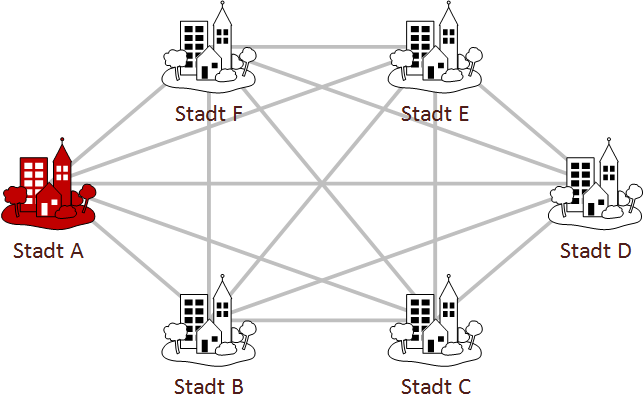
\includegraphics[width=0.9\linewidth]{images/TSP_ACO_numerisch.png}
		\caption{Darstellung des \ac{TSP}-Beispiels zur Darlegung der Arbeitsweise der Architektur}
		\label{tspAcoNumerisch}
	\end{figure}

	Nun wird die gleiche Berechnung aufgezeigt, welche die Applikation durchführen würde. In Tabelle \ref{tspAcoNumerisch_matrix} zu sehen ist die allgemeingültige Streckenmatrix für das vorliegende Beispiel. Innerhalb der Matrix sind jeweils die Streckenlängen von einer Stadt zur Anderen gespeichert. So besitzt die Strecke von D nach C die Länge 4\footnote{Hier könnte natürlich eine beliebige Längeneinheit ergänzt werden. Dies ist aber für das Lösen des Problems und das Beschreiben des Vorgehens nicht notwendig und wird deswegen weggelassen.}. Auffällig sind die Strecken von den Städten zu sich selbst, welche mit -1 gekennzeichnet sind. Diese Zahl wird später für die Applikation ein Hinweis sein, dass ein Fehler vorliegt und dieser korrigiert werden muss.
	
	\begin{table}
		\centering
		\footnotesize
		\setstretch{0.75}
		\begin{tabular}{c c c c c c c}
			  & A & B & C & D & E & F \\
			A & -1 & 3 & 9 & 13 & 11 & 5\\ 
			B & 3 & -1 & 7 & 10 & 9 & 8\\ 
			C & 9 & 7 & -1 & 4 & 6 & 10\\
			D & 13 & 10 & 4 & -1 & 2 & 12\\
			E & 11 & 9 & 6 & 2 & -1 & 8\\
			F & 5 & 8 & 10 & 12 & 8 & -1\\
		\end{tabular}
		\caption{Distanzmatrix des \ac{TSP}-Beispiels}
		\label{tspAcoNumerisch_matrix}
	\end{table}

	Besonders wichtig für die Berechnung der \ac{ACO}-Lösung ist die Pheromonmatrix, welche in Tabelle \ref{tspAcoNumerisch_pheromon_initial} im initialisierten Zustand gezeigt ist. Die Normalisierung mit einem durchgängigen Wert von 1 bewirkt, dass im ersten Durchlauf die Pheromone keinerlei Einfluss auf die Entscheidungen der Ameisen haben. Dies entspricht dem Umstand einer neu aufgebauten Ameisenkolonie, welche sich erst zurecht finden muss.
	
	\begin{table}
		\centering
		\footnotesize
		\setstretch{0.75}
		\begin{tabular}{c c c c c c c}
			& A & B & C & D & E & F \\
			A & 1 & 1 & 1 & 1 & 1 & 1\\ 
			B & 1 & 1 & 1 & 1 & 1 & 1\\ 
			C & 1 & 1 & 1 & 1 & 1 & 1\\
			D & 1 & 1 & 1 & 1 & 1 & 1\\
			E & 1 & 1 & 1 & 1 & 1 & 1\\
			F & 1 & 1 & 1 & 1 & 1 & 1\\
		\end{tabular}
		\caption{Initiale Pheromonmatrix des \ac{TSP}-Beispiels}
		\label{tspAcoNumerisch_pheromon_initial}
	\end{table}

	Mit den vorliegenden Daten, der Streckenlängenmatrix und der initialen Matrix, kann nun das \ac{TSP} mithilfe von \ac{ACO} berechnet werden. In diesem Beispiel werden drei Ameisen verwendet, um das Verhalten zeigen zu können, aber gleichzeitig den Aufwand gering zu halten.
	
	Jede Ameise startet bei der Kolonie, welche bei Stadt A liegt. Daher muss für jede Ameise jetzt ausgewählt werden, wohin diese gehen soll. Für jede mögliche Strecke wird nun eine Variabel berechnet, welche im Folgenden mit $\lambda$ \footnote{Mehr zu diesen beiden Werten in Kapitel \ref{parameter}.} bezeichnet wird. $\lambda$ setzt sich zusammen aus dem Pheromonwert der betrachteten Strecke und der zugehörigen Streckenlänge.

	Nun wird für jede Ameise einzeln betrachtet, welche Städte noch erreichbar sind - also noch nicht besucht sind - und welchen Wert $\lambda$ für die Strecke zu dieser Stadt besitzt. $\lambda$ einer Stadt wird dann mit der Summe aus den $\lambda$ aller erreichbaren Städten verglichen. Hierdurch wird ein Wert - im Folgenden mit $\rho$ referenziert - erzeugt, welcher zwischen 0 und 1 liegt. 
	
	Um nun bestimmen zu können, welche Ameise welchen Weg wählt, wird eine Zufallszahl $n$ bestimmt, welche ebenfalls zwischen 0 und 1 liegt. Nacheinander wird für alle erreichbaren Städte nun verglichen, ob sich $\rho>n$ ergibt. Sobald eine Stadt die Gleichung erfüllt, wählt die Ameise diesen Weg und zieht weiter. Erfüllt keine Stadt diese Gleichung so werden nacheinander die $\rho$ der Städte aufaddiert, bis eine Stadt x die Gleichung $n < \sum_x^{} \rho$ erfüllt. Wenn diese Gleichung erfüllt ist, wählt die Ameise der Strecke zu Stadt x.
	
	In dem vorliegenden Beispiel bedeutet das, dass von Stadt A aus alle möglichen Strecken ausgewertet werden. Folgend ist die Berechnung von $\lambda$ aller erreichbaren Städte aufgezeigt.
	\begin{equation}
		A -> B \quad (1)^2 * (\frac{1}{3}) = \frac{1}{3}
	\end{equation}
	\begin{equation}
		A -> C \quad (1)^2 * (\frac{1}{5}) = \frac{1}{5}
	\end{equation}
	\begin{equation}
		A -> D \quad (1)^2 * (\frac{1}{9}) = \frac{1}{9}
	\end{equation}
	\begin{equation}
		A -> E \quad (1)^2 * (\frac{1}{13}) = \frac{1}{13}
	\end{equation}
	\begin{equation}
		A -> F \quad (1)^2 * (\frac{1}{11}) = \frac{1}{11}
	\end{equation}
	\myequations{Formeln zum Berechnen des Verhältnisses $\lambda$ von Pheromonwert und Streckenlänge}
	
	Aus diesen kann nun $\rho$ errechnet werden, in dem alle $\lambda$ durch die Summe aller $\lambda$ - welche 0,812 beträgt - dividiert werden. $\rho$ steht dann für die Wahrscheinlichkeit, dass dieser Weg gewählt wird. Somit ergeben sich folgende fünf Wahrscheinlichkeiten:
	\begin{equation}
		\rho(AB) = \frac{\frac{1}{3}}{0,8122} = 0.410
	\end{equation}
	\begin{equation}
		\rho(AC) = \frac{\frac{1}{5}}{0,8122} = 0.136
	\end{equation}
	\begin{equation}
		\rho(AD) = \frac{\frac{1}{9}}{0,8122} = 0.094
	\end{equation}
	\begin{equation}
		\rho(AE) = \frac{\frac{1}{13}}{0,8122} = 0.111
	\end{equation}
	\begin{equation}
		\rho(AF) = \frac{\frac{1}{11}}{0,8122} = 0.246
	\end{equation}
	\myequations{Formeln zum Berechnen der Wahrscheinlichkeiten $\rho$ aus dem Verhältnis $\lambda$ und der Summe aller $\lambda$}
	
	Nun muss für jede der drei Ameisen eine Zufallszahl bestimmt werden, welche mit $\rho$ verglichen werden kann. Es wurden die Zahlen 0.242 für Ameise 1, 0.033 für Ameise 2 und 0.455 für Ameise 3 errechnet.
	Nach dem bereits beschriebenen Vorgehen wählen Ameise 1 und Ameise 2 nun die Stadt B als Zielstadt. Ameise 3 wählt Stadt C, da der Zufallswert zu groß war um eine direkte Auswahl zu treffen. Ein Aufaddieren der Werte $\rho(AB)$ und $\rho(AC)$ hat allerdings schon ausgereicht, um den Wert zu überschreiten.
	
	Diesen Vorgehen kann nun für alle Städte wiederholt werden, sodass am Ende alle Ameisen alle Städte besucht haben und auch wieder in der Anfangsstadt in der Kolonie angekommen sind. Nun muss noch die Pheromonmatrix aktualisiert werden, um der Kolonie mitzuteilen welche Wege profitable sind. Hierbei wird von jeder Ameise auf jedem Weg den sie ablaufen konstant Pheromone abgegeben. Dadurch ergibt sich als zusätzlicher Pheromonwert die der Kehrwert der Streckenlänge. Der Kehrwert wird auf den aktuellen Wert in der Pheromonmatrix addiert, wodurch die nächste Generation diese in die Berechnung einbeziehen kann.
	
	In Tabelle \ref{tspAcoNumerisch_ergebnis_1} zu erkennen sind die kompletten Wegstrecken, die die Ameisen gewählt haben. Aus dieser Liste ableiten lassen sich nun die zusätzlichen Pheromonwerte, in dem man die Tabelle \ref{tspAcoNumerisch_matrix} miteinbezieht. Addiert man die zusätzlichen Pheromonwerte auf die vorherige Pheromonmatrix, so erhält man die in Tabelle \ref{tspAcoNumerisch_pheromon_1} gezeigte neue  Pheromonmatrix.
	
	\begin{table}
		\centering
		\footnotesize
		\setstretch{0.75}
		\begin{tabular}{l c r}
			Ameise & Weglänge & Wegstrecke \\
			1 & 40 & A, B, F, D, E, C, A\\
			2 & 36 & A, B, F, E, D, C, A\\ 
			3 & 50 & A, C, D, B, F, E, A\\
		\end{tabular}
		\caption{Ergebnisse der drei Ameisen der ersten Generation}
		\label{tspAcoNumerisch_ergebnis_1}
	\end{table}
	
	\begin{table}
		\centering
		\footnotesize
		\setstretch{0.75}
		\begin{tabular}{c c c c c c c}
			& A & B & C & D & E & F \\
			A & 1 & $\frac{5}{3}$ & $\frac{10}{9}$ & 1 & 1 & 1\\ 
			B & 1 & 1 & 1 & 1 & 1 & $\frac{5}{4}$\\ 
			C & $\frac{11}{9}$ & 1 & 1 & $\frac{5}{4}$ & 1 & 1\\
			D & 1 & $\frac{11}{10}$ & $\frac{5}{4}$ & 1 & $\frac{3}{2}$ & 1\\
			E & $\frac{12}{11}$ & 1 & $\frac{7}{6}$ & $\frac{3}{2}$ & 1 & 1\\
			F & 1 & 1 & 1 & $\frac{13}{12}$ & $\frac{5}{4}$ & 1\\
		\end{tabular}
		\caption{Pheromonmatrix des TSP-Beispiels nach dem ersten Durchlauf}
	\label{tspAcoNumerisch_pheromon_1}
	\end{table}

	Nach der Berechnung der neuen Pheromonmatrix ist die erste Generation der Ameisen abgeschlossen. Nun werden sich drei neue Ameisen auf die Reise begeben. Da die Pheromonmatrix nicht mehr normalisiert ist, sondern von 1 abweichende Werte enthält, können die neuen Ameisen die Pheromonmatrix effektiv in die Berechnung der Wahrscheinlichkeiten miteinbeziehen. So wird beispielsweise $\lambda$ für die Strecke A - B nun mit folgender Gleichung berechnet:	
	\begin{equation}
		A -> B \quad (\frac{5}{3})^2 * (\frac{1}{3})
	\end{equation}
	Hierbei wird nun das Verhältnis zwischen Pheromonen und Streckenlänge betrachtet, wobei die Pheromone doppelt so schwer gewichtet werden. Die restliche Berechnung läuft allerdings parallel zum vorherigen Vorgehen ab. Die zweite Generation der Ameisen hat, wie man aus dem Vergleich zwischen Tabelle \ref{tspAcoNumerisch_ergebnis_1} und Tabelle \ref{tspAcoNumerisch_ergebnis_2} erkennt, bei einigen Strecken eine andere Wahl getroffen. Im Durchschnitt ist neue Generation auch schneller voran gekommen, was an den Weglängen - also der Summe aller gelaufenen Strecken - erkennbar ist.
	
	\begin{table}
		\centering
		\footnotesize
		\setstretch{0.75}
		\begin{tabular}{l c r}
			Ameise & Weglänge & Wegstrecke \\
			1 & 40 & A, C, E, D, B, F, A\\
			2 & 29 & A, F, E, D, C, B, A\\ 
			3 & 41 & A, F, E, D, B, C, A\\
		\end{tabular}
		\caption{Ergebnisse der drei Ameisen der zweiten Generation}
		\label{tspAcoNumerisch_ergebnis_2}
	\end{table}
	
	Auch diese Generation verteilt auf allen besuchten Strecken ihre Pheromone, was wieder zu einer Aktualisierung der Pheromonmatrix führt. In Tabelle \ref{tspAcoNumerisch_pheromon_2} zu erkennen ist, dass nun deutlich mehr Streckenabschnitte besucht wurden und einen von 1 abweichenden Pheromonwert besitzen.
	
	\begin{table}
		\centering
		\footnotesize
		\setstretch{0.75}
		\begin{tabular}{c c c c c c c}
			& A & B & C & D & E & F \\
			A & 1 & $\frac{5}{3}$ & $\frac{11}{9}$ & 1 & 1 & $\frac{7}{5}$\\ 
			B & $\frac{4}{3}$ & 1 & $\frac{8}{7}$ & 1 & 1 & $\frac{11}{8}$\\ 
			C & $\frac{4}{3}$ & $\frac{11}{10}$ & 1 & $\frac{5}{4}$ & $\frac{7}{6}$ & 1\\
			D & 1 & $\frac{13}{10}$ & $\frac{3}{2}$ & 1 & $\frac{3}{2}$ & 1\\
			E & $\frac{12}{11}$ & 1 & $\frac{7}{6}$ & 3 & 1 & 1\\
			F & $\frac{6}{5}$ & 1 & 1 & $\frac{13}{12}$ & $\frac{3}{2}$ & 1\\
		\end{tabular}
		\caption{Pheromonmatrix des \ac{TSP}-Beispiels nach dem zweiten Durchlauf}
		\label{tspAcoNumerisch_pheromon_2}
	\end{table}

	Nach der zweiten Generation macht sich noch eine letzte Generation der Ameisen auf den Weg und läuft wieder die gleichen Orte ab. Wieder wird die vorher aktualisierte Pheromonmatrix in die Gewichtung miteinbezogen, um ein effizienteres Ergebnis zu erhalten. Betrachtet man das in Tabelle \ref{tspAcoNumerisch_ergebnis_3} gezeigte Ergebnis der Ameisen, so ist deutlich sichtbar dass eine Verbesserung vorliegt. Alle Ameisen kamen schneller voran, als ihre Vorgänger. 
	
	\begin{table}
		\centering
		\footnotesize
		\setstretch{0.75}
		\begin{tabular}{l c r}
			Ameise & Weglänge & Wegstrecke \\
			1 & 35 & A, B, C, E, D, F, A\\
			2 & 33 & A, B, E, D, C, F, A\\ 
			3 & 29 & A, B, C, D, E, F, A\\
		\end{tabular}
		\caption{Ergebnisse der drei Ameisen der dritten Generation}
		\label{tspAcoNumerisch_ergebnis_3}
	\end{table}

	\begin{table}
		\centering
		\footnotesize
		\setstretch{0.75}
		\begin{tabular}{c c c c c c c}
			& A & B & C & D & E & F \\
			A & 1 & $\frac{8}{3}$ & $\frac{11}{9}$ & 1 & 1 & $\frac{7}{5}$\\ 
			B & $\frac{4}{3}$ & 1 & $\frac{10}{7}$ & 1 & $\frac{10}{9}$ & $\frac{11}{8}$\\ 
			C & $\frac{4}{3}$ & $\frac{11}{10}$ & 1 & $\frac{3}{2}$ & $\frac{8}{6}$ & $\frac{11}{10}$\\
			D & 1 & $\frac{13}{10}$ & $\frac{7}{4}$ & 1 & 2 & $\frac{13}{12}$\\
			E & $\frac{12}{11}$ & 1 & $\frac{7}{6}$ & 4 & 1 & $\frac{9}{8}$\\
			F & $\frac{9}{5}$ & 1 & 1 & $\frac{13}{12}$ & $\frac{3}{2}$ & 1\\
		\end{tabular}
		\caption{Pheromonmatrix des \ac{TSP}-Beispiels nach dem finalen dritten Durchlauf}
		\label{tspAcoNumerisch_pheromon_3}
	\end{table}

	Abschließend lässt sich aus der finale Pheromonmatrix - in Tabelle \ref{tspAcoNumerisch_pheromon_3} gezeigt - erkennen, dass zum Einen ein Großteil der Strecken besucht wurde. Zum Anderen liegt bereits nach drei Generationen teilweise eine deutliche Gewichtung vor, sodass bei Stadt E meist nur noch die Stadt D gewählt wird.
	Es lässt sich bereits bei dieser manuellen Berechnung schlussfolgern, dass mehr Ameisen lediglich bedeuten, dass die Pheromonverteilung schneller angepasst und optimiert wird. Dies hat zur Folge, dass bei höherer Ameisenzahl weniger Generationen benötigt werden, um ein besseres Ergebnis zu erhalten. Allerdings hat es keinen Einfluss auf das Endergebnis.